% This is a basic Math Paper

\documentclass[11pt]{article}

% Preamble

\usepackage[margin=1in]{geometry}
\usepackage{amsfonts, amsmath, amssymb}
\usepackage{fancyhdr, float, graphicx}
%\usepackage[utf8]{inputenc} % Required for inputting international characters
%\usepackage[T1]{fontenc} % Output font encoding for international characters
%\usepackage{fouriernc} % Use the New Century Schoolbook font
\usepackage[nottoc, notlot, notlof]{tocbibind}
\usepackage[hidelinks]{hyperref}
%\usepackage{helvet}
% Header and Footer
\pagestyle{fancy}
\fancyhead{}
\fancyfoot{}
\fancyhead[L]{\textit{\Large{Demonstration of Refrigeration Test Rig}}}
%\fancyhead[R]{\textit{something}}
\fancyfoot[C]{\thepage}
\renewcommand{\footrulewidth}{1pt}



% Other Doc Editing
% \parindent 0ex
%\renewcommand{\baselinestretch}{1.5}

\begin{document}
	
	\begin{titlepage} 
		\centering 
		
		%---------------------------NAMES-------------------------------
		
		\huge\textsc{
			MIT World Peace University
		}\\
	
		\vspace{0.75\baselineskip} % space after Uni Name
		
		\LARGE{
			Basic Mechanical Engineering\\
			First Year B. Tech, Trimester 1
		}
		
		\vfill % space after Sub Name
		
		%--------------------------TITLE-------------------------------
		
		\rule{\textwidth}{1.6pt}\vspace*{-\baselineskip}\vspace*{2pt}
		\rule{\textwidth}{0.6pt}
		\vspace{0.4\baselineskip} % Whitespace above the title
		
		
		
		\huge{\textsc{
				Demonstration of a Refrigeration Test Rig
			}} \\
		
		
		
		\vspace{0.5\baselineskip} % Whitespace below the title
		\rule{\textwidth}{0.6pt}\vspace*{-\baselineskip}\vspace*{2.8pt}
		\rule{\textwidth}{1.6pt}
		
		\vspace{1\baselineskip} % Whitespace after the title block

		%--------------------------SUBTITLE --------------------------	
			
		\LARGE\textsc{
			Experiment Number 6\\Practical Report
		} % Subtitle or further description
		\vfill
		
		%--------------------------AUTHOR-------------------------------
		
		Prepared By
		\vspace{0.5\baselineskip} % Whitespace before the editors
		
		\Large{
			Krishnaraj Thadesar \\
			Division 9, Roll No. 54
		}
		
		
		\vspace{0.5\baselineskip} % Whitespace below the editor list
		\today

	\end{titlepage}
	
	
\tableofcontents
\thispagestyle{empty}
\clearpage
\setcounter{page}{1}

\section{Objective}
To Study and understand the working principle and components of refrigerator.


\section{Theory}

Refrigeration is defined as an art of producing and maintaining temperature in a space below atmospheric temperature. A refrigerator is equipment used to remove the heat continuously from space (Sink) and maintain the temperature below atmospheric temperature and reject heat to the atmosphere (source).

\subsection{Artificial methods of obtaining refrigeration}

Conveyor systems are used widespread across a range of industries due to the numerous benefits they provide.


\begin{enumerate}
	\item Vapour compression cycle
	\item Vapour absorption cycle
	\item Air or Gas cycle refrigeration
	\item Steam jet refrigeration
	\item Non-conventional Methods
\end{enumerate}

\subsection{Working of the Refrigerator}

The first two methods are used extensively on commercial basis. The first method i.e. “Vapour Compression Cycle” is most widely used system worldwide and we will limit our scope of study to this method only.\\


For obtaining refrigeration, heat is to be removed from a substance or space maintained at a lower temperature. In order to absorb this heat at lower temperature, the working medium, the refrigerant liquid, has to boil at the temperature lower than the space temperature so that it absorbs the latent heat from the refrigerated space. The heat exchanger placed inside the refrigerated space is called evaporator as the refrigerant liquid evaporates here. The pressure of the refrigerant liquid has to be low enough so that it can boil at lower temperature.  
(See figure:\ref{fig:Refrigeration System})\\


The vapour coming from the evaporator is at a low temperature and low pressure. In order to reuse the same refrigerant in the evaporator, it has to undergo a cyclic process. A compressor is used to raise the temperature and pressure. The compressor achieves two functions – it continuously sucks and removes vapour from the evaporator thus maintaining a low pressure in the evaporator, and it also raises the temperature and pressure of the vapour so that it can reject heat in the condenser.\\


Due to high pressure after compression, the condensing temperature of the refrigerant increases above the surrounding ambient temperature. Condenser is also a heat exchanger like the evaporator. The high temperature high pressure vapour flows on one side and ambient air or water flows on the other side. The temperature of refrigerant vapour is higher than the surrounding medium (ambient air/water), so it rejects heat to this medium and gets cooled down to its saturation temperature and further rejection of heat condenses it to liquid. At the outlet of the condenser, the refrigerant is high temperature, high pressure liquid.\\

\begin{figure}[H]
	\centering
	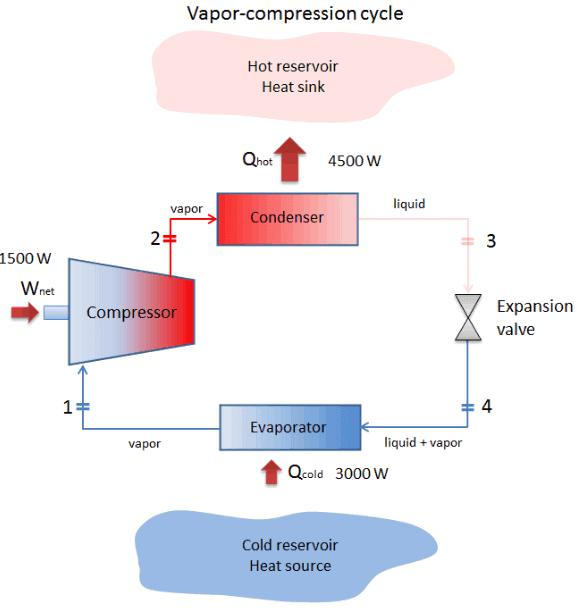
\includegraphics[scale=0.6]{Refrigeration system.jpg}
	\caption{Basic Components of a Refrigeration System\cite{VP cycle}}
	\label{fig:Refrigeration System}
\end{figure}



This high temperature high pressure liquid is made to flow through a restricted path which causes the pressure drop. Expansion device is the component used to create obstruction to flow of liquid and also to meter the refrigerant flow through the evaporator in response to varying load. The expansion device could be a capillary tube or a thermostatic expansion valve. When the high temperature high pressure liquid flows through the expansion device, its pressure drops to the evaporator pressure and the temperature also is lowered. The process occurs without any heat or work exchange and is called throttling. In throttling a small part of liquid is converted to vapour, this is called flashing.


This low temperature, low pressure liquid with a small amount of vapour enters the evaporator for extracting heat from low temperature surrounding. The cycle repeats.
\pagebreak

\subsection{Refrigeration Effect and COP}

Refrigeration effect is the removal of heat from a body or space at low temperature. This occurs in evaporator. The amount of heat extracted at low temperature in the evaporator is called the refrigeration effect. Work is required to be done on the refrigerant to compress it. The net work input is the net work required for the compression. The performance of a refrigeration system can be evaluated by taking a
ratio of refrigeration effect to net work input. \textit{This is termed as Coefficient of Performance or COP}


\subsection{Theoretical Simple Saturated Vapour Compression Cycle}

The four processes in a theoretical Vapour Compression Cycle are:

\begin{enumerate}
	\item 1-2: Reversible adiabatic or isentropic compression of refrigerant vapour.
	\item 1-2: Reversible adiabatic or isentropic compression of refrigerant vapour.
	\item 3-4: Irreversible expansion at constant enthalpy – (throttling)
	\item 4-1: Reversible heat absorption at constant pressure (evaporation from liquid to vapour)
	
	(see figure: \ref{fig:PH graph})
\end{enumerate}

\begin{figure}[H]
	\centering
	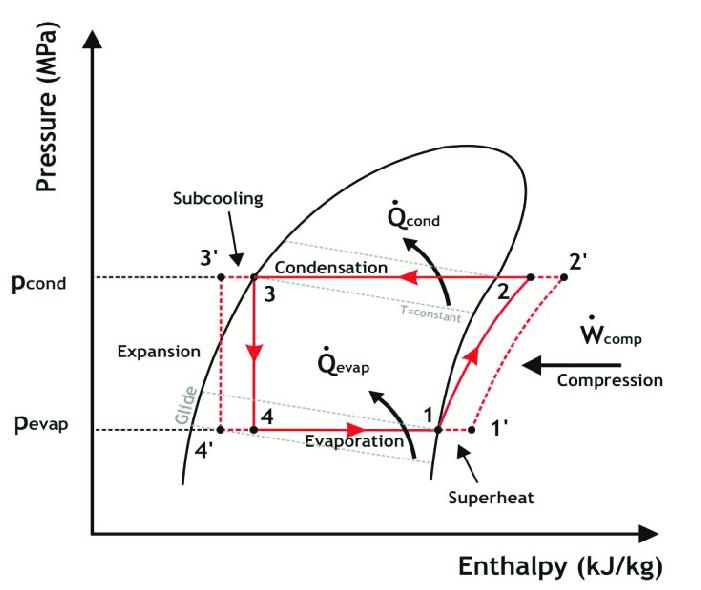
\includegraphics[scale=0.5]{PH graph.jpg}
	\caption{Pressure and Enthalpy Graph \cite{ph graph}}
	\label{fig:PH graph}
\end{figure}

\pagebreak

Heat rejected in condenser = \\
$$ QR = q_2 - q_3 = (h_2-h_3)\ \ldots\ \mathrm{on\ unit\ basis}$$

Refrigeration effect = Heat absorbed in evaporator = 
$$QA = q_4-q_1 = (h_1-h_4)$$

Net work input, Win = Heat rejected - Heat absorbed = 
$$QR - QA = (h_2-h_3) - (h_1-h_4) = (h_2-h_1)$$

$$COP = \frac{\mathrm{Refrigeration\ Effect}}{\mathrm{Net\ Work\ Input}} = \frac{h_1-h_4}{h_2-h_1}$$

\subsection{Domestic Refrigerator}
The basic components are: 

\begin{enumerate}
\item \textit{Evaporator and Compressor:} The evaporator (part of the freezer cabinet) where the refrigerant (working fluid) evaporates absorbs the latent heat of vaporization. In modern frost free refrigerators, the evaporator is located outside the cabinet, as fan circulates air from evaporator to the freezer. Just below the freezer, there is a chiller tray. Further below are compartments with progressive higher temperature. The cold air being heavier flows down from the freezer to the bottom of the refrigerator. The warm air being lighter flows upward from vegetable box to freezer gets cooled and flows down again. Thus natural convection current is set up which maintains a temperature gradient between top and bottom of refrigerator. The temperature maintained in the freezer is - 15°C. \\

\item \textit{Condenser}: The condenser is usually a wire and tube type mounted at the back of the refrigerator. Having no fan, the refrigerator vapor is condensed with the help
of surrounding air which rises above by natural convection as it gets heated after absorbing the latent heat of condensation from refrigerant. After condensation, the high pressure liquid refrigerant is reduced to the low pressure of the evaporator by passing through liquid.

\item \textit{Expansion device:} Refrigerant is reduced to the low pressure of the evaporator by passing through an expansion device (throttle) valve or capillary tube and cycle is completed.

\end{enumerate}




\section{Conclusion}
	
The Working and applications of a Refrigeration Rig were studied and understood in detail. 

\pagebreak

\section{Questions}
\parindent 0ex
Q1. Define Refrigerant, COP and Tons of Refrigeration \\
A1. 
\begin{enumerate}
	\item Refrigerant: A refrigerant is a working fluid used in the refrigeration cycle of air conditioning systems and heat pumps where in most cases they undergo a repeated phase transition from a liquid to a gas and back again. Refrigerants are heavily regulated due to their toxicity, flammability and the contribution of CFC and HCFC refrigerants to ozone depletion and that of HFC refrigerants to climate change.
	
	\item COP: The performance of a refrigeration system can be evaluated by taking a
	ratio of refrigeration effect to net work input. \textit{This is termed as Coefficient of Performance or COP}
	$$COP = \frac{\mathrm{Refrigeration\ Effect}}{\mathrm{Net\ Work\ Input}} = \frac{h_1-h_4}{h_2-h_1}$$
	
	
	
	\item Tons of Refrigeration: A ton of refrigeration (TR or TOR), also called a refrigeration ton (RT), is a unit of power used in some countries (especially in North America) to describe the heat-extraction capacity of refrigeration and air conditioning equipment. It is defined as the rate of heat transfer that results in the freezing or melting of 1 short ton (2,000 lb; 907 kg) of pure ice at 0 °C (32 °F) in 24 hours\\
\end{enumerate}



Q2. Explain with a neat sketch the principle and working of a household refrigerator.\\
A2. A refrigerator works in the following steps:


\begin{figure}[H]
	\centering
	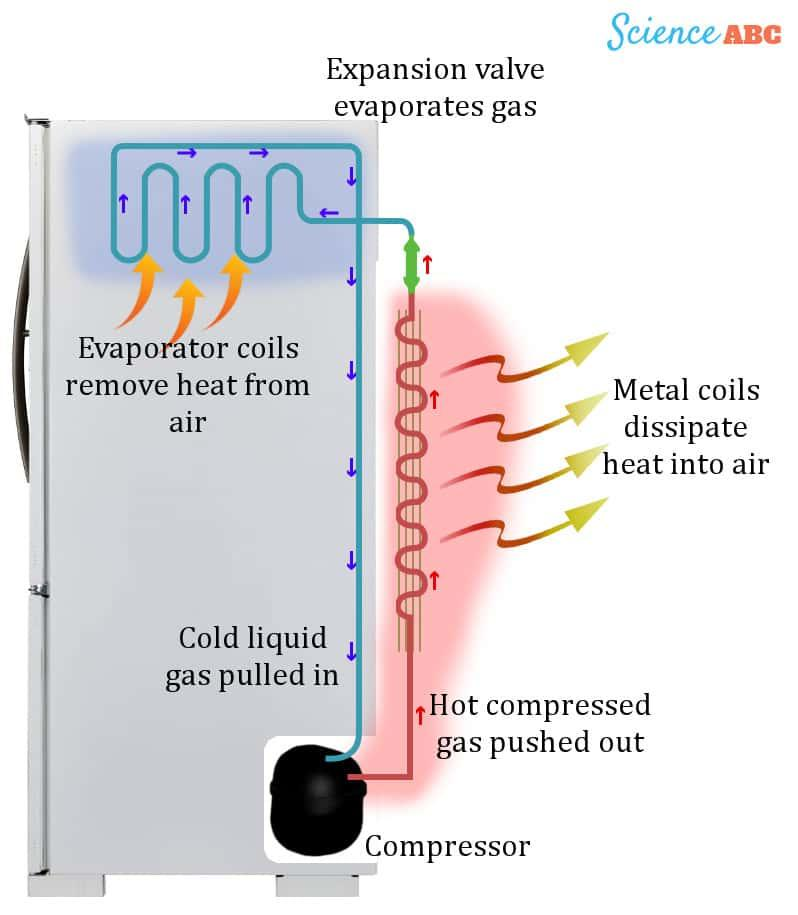
\includegraphics[scale=0.3]{household refrigerator.jpg}
	\caption{Working of a household Refrigerator \cite{household refrigerator}}
	\label{fig:Working of a Refrigerator}
	
\end{figure}



\begin{enumerate}
\item The \textit{compressor} compresses the refrigerant gas. The compressed gas heats up as it is pressurized.
\item The coils on the back of the refrigerator let the hot refrigerant gas dissipate its heat. The refrigerant gas condenses into liquid at high pressure. These coils are what we call the\textit{ Condenser}.
\item The high-pressure liquid at about 8 bar flows through the \textit{expansion valve}.
The liquid immediately boils and vaporizes, its temperature dropping to about -20 °C and about 0.6 bar Pressure. As the cold gas flows through the expansion coils (inside the refrigerator, called \textit{the Evaporator}) it makes the inside cold by absorbing heat.
\item The low pressure refrigerant gas is sucked up by the compressor, and the cycle repeats.
\end{enumerate}



Q3. Explain with a neat sketch the principle and working of an A/C.\\
A3. When you turn on an air conditioner and set the desired temperature, say 20 degrees Celsius, the thermostat installed in it will detect that there is a difference between the temperature of the room air and the temperature you have chosen.\\


\begin{figure}[H]
	\centering
	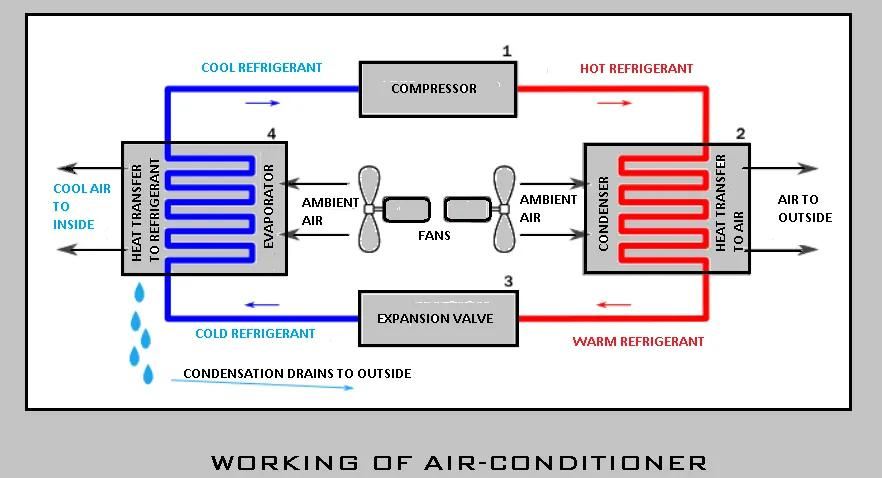
\includegraphics[scale=0.5]{AC.jpg}
	\caption{Working of an AC \cite{AC}}
	\label{fig:Working of an AC}
\end{figure}


This warm air is sucked in through a grill at the bottom of the indoor unit, which then flows through some pipes through which the refrigerant, i.e. a coolant, flows. The refrigerant fluid absorbs the heat and itself becomes a hot gas. Thus, heat is removed from the air that falls on the evaporator coils. Note that the evaporator coil not only absorbs heat, but also flushes moisture out of the incoming air, which helps to dehumidify the room.\\

This hot refrigerant gas is then passed on to the compressor located on the outside unit. True to its name, the compressor compresses the gas so that it becomes hot as the compression of a gas increases its temperature.\\

This hot high-pressure gas then reaches the third component – the condenser. Here, too, the condenser stays true to its name and condenses the hot gas into a liquid.\\

The refrigerant enters the condenser as a hot gas but quickly becomes a cooler liquid because the heat from the “hot gas” is dissipated into the environment through metal fins. As a result, the refrigerant loses its heat as it leaves the condenser and becomes a cooler liquid. This flows through an expansion valve – a tiny hole in the system’s copper tube – which controls the flow of the cool liquid refrigerant into the evaporator, so that the refrigerant arrives at the point where its journey began.


\pagebreak
\begin{thebibliography}{}


\bibitem{VP cycle}
"What is Vapor-compression Cycle – Refrigeration Cycle – Definition"

\url{https://www.thermal-engineering.org/what-is-vapor-compression\\-cycle-refrigeration-cycle-definition/}\\
Image taken from website
	
\bibitem{ph graph}
"PH Diagram of the Vapour Compression Refrigeration Cycle"

\url{https://www.researchgate.net/figure/P-h-diagram-of-the-vapour\\-compression-refrigeration-cycle-considered-in-Fig-1_fig3_316144041}\\
Image taken from this website


\bibitem{household refrigerator}
"Working of a Refrigerator"

\url{https://www.scienceabc.com/innovation/how-does-a-refrigerator\\-work-working-principle.html}\\
Image taken from this website
	
	
\bibitem{AC}
"Working of an Air Conditioner"

\url{https://www.scienceabc.com/innovation/air-conditioner-ac-work.html}\\
Image taken from this website
	

	
	
\end{thebibliography}
	
	
\end{document}